% Options for packages loaded elsewhere
\PassOptionsToPackage{unicode}{hyperref}
\PassOptionsToPackage{hyphens}{url}
%
\documentclass[
]{article}
\usepackage{amsmath,amssymb}
\usepackage{iftex}
\ifPDFTeX
  \usepackage[T1]{fontenc}
  \usepackage[utf8]{inputenc}
  \usepackage{textcomp} % provide euro and other symbols
\else % if luatex or xetex
  \usepackage{unicode-math} % this also loads fontspec
  \defaultfontfeatures{Scale=MatchLowercase}
  \defaultfontfeatures[\rmfamily]{Ligatures=TeX,Scale=1}
\fi
\usepackage{lmodern}
\ifPDFTeX\else
  % xetex/luatex font selection
\fi
% Use upquote if available, for straight quotes in verbatim environments
\IfFileExists{upquote.sty}{\usepackage{upquote}}{}
\IfFileExists{microtype.sty}{% use microtype if available
  \usepackage[]{microtype}
  \UseMicrotypeSet[protrusion]{basicmath} % disable protrusion for tt fonts
}{}
\makeatletter
\@ifundefined{KOMAClassName}{% if non-KOMA class
  \IfFileExists{parskip.sty}{%
    \usepackage{parskip}
  }{% else
    \setlength{\parindent}{0pt}
    \setlength{\parskip}{6pt plus 2pt minus 1pt}}
}{% if KOMA class
  \KOMAoptions{parskip=half}}
\makeatother
\usepackage{xcolor}
\usepackage[margin=1in]{geometry}
\usepackage{color}
\usepackage{fancyvrb}
\newcommand{\VerbBar}{|}
\newcommand{\VERB}{\Verb[commandchars=\\\{\}]}
\DefineVerbatimEnvironment{Highlighting}{Verbatim}{commandchars=\\\{\}}
% Add ',fontsize=\small' for more characters per line
\usepackage{framed}
\definecolor{shadecolor}{RGB}{248,248,248}
\newenvironment{Shaded}{\begin{snugshade}}{\end{snugshade}}
\newcommand{\AlertTok}[1]{\textcolor[rgb]{0.94,0.16,0.16}{#1}}
\newcommand{\AnnotationTok}[1]{\textcolor[rgb]{0.56,0.35,0.01}{\textbf{\textit{#1}}}}
\newcommand{\AttributeTok}[1]{\textcolor[rgb]{0.13,0.29,0.53}{#1}}
\newcommand{\BaseNTok}[1]{\textcolor[rgb]{0.00,0.00,0.81}{#1}}
\newcommand{\BuiltInTok}[1]{#1}
\newcommand{\CharTok}[1]{\textcolor[rgb]{0.31,0.60,0.02}{#1}}
\newcommand{\CommentTok}[1]{\textcolor[rgb]{0.56,0.35,0.01}{\textit{#1}}}
\newcommand{\CommentVarTok}[1]{\textcolor[rgb]{0.56,0.35,0.01}{\textbf{\textit{#1}}}}
\newcommand{\ConstantTok}[1]{\textcolor[rgb]{0.56,0.35,0.01}{#1}}
\newcommand{\ControlFlowTok}[1]{\textcolor[rgb]{0.13,0.29,0.53}{\textbf{#1}}}
\newcommand{\DataTypeTok}[1]{\textcolor[rgb]{0.13,0.29,0.53}{#1}}
\newcommand{\DecValTok}[1]{\textcolor[rgb]{0.00,0.00,0.81}{#1}}
\newcommand{\DocumentationTok}[1]{\textcolor[rgb]{0.56,0.35,0.01}{\textbf{\textit{#1}}}}
\newcommand{\ErrorTok}[1]{\textcolor[rgb]{0.64,0.00,0.00}{\textbf{#1}}}
\newcommand{\ExtensionTok}[1]{#1}
\newcommand{\FloatTok}[1]{\textcolor[rgb]{0.00,0.00,0.81}{#1}}
\newcommand{\FunctionTok}[1]{\textcolor[rgb]{0.13,0.29,0.53}{\textbf{#1}}}
\newcommand{\ImportTok}[1]{#1}
\newcommand{\InformationTok}[1]{\textcolor[rgb]{0.56,0.35,0.01}{\textbf{\textit{#1}}}}
\newcommand{\KeywordTok}[1]{\textcolor[rgb]{0.13,0.29,0.53}{\textbf{#1}}}
\newcommand{\NormalTok}[1]{#1}
\newcommand{\OperatorTok}[1]{\textcolor[rgb]{0.81,0.36,0.00}{\textbf{#1}}}
\newcommand{\OtherTok}[1]{\textcolor[rgb]{0.56,0.35,0.01}{#1}}
\newcommand{\PreprocessorTok}[1]{\textcolor[rgb]{0.56,0.35,0.01}{\textit{#1}}}
\newcommand{\RegionMarkerTok}[1]{#1}
\newcommand{\SpecialCharTok}[1]{\textcolor[rgb]{0.81,0.36,0.00}{\textbf{#1}}}
\newcommand{\SpecialStringTok}[1]{\textcolor[rgb]{0.31,0.60,0.02}{#1}}
\newcommand{\StringTok}[1]{\textcolor[rgb]{0.31,0.60,0.02}{#1}}
\newcommand{\VariableTok}[1]{\textcolor[rgb]{0.00,0.00,0.00}{#1}}
\newcommand{\VerbatimStringTok}[1]{\textcolor[rgb]{0.31,0.60,0.02}{#1}}
\newcommand{\WarningTok}[1]{\textcolor[rgb]{0.56,0.35,0.01}{\textbf{\textit{#1}}}}
\usepackage{longtable,booktabs,array}
\usepackage{calc} % for calculating minipage widths
% Correct order of tables after \paragraph or \subparagraph
\usepackage{etoolbox}
\makeatletter
\patchcmd\longtable{\par}{\if@noskipsec\mbox{}\fi\par}{}{}
\makeatother
% Allow footnotes in longtable head/foot
\IfFileExists{footnotehyper.sty}{\usepackage{footnotehyper}}{\usepackage{footnote}}
\makesavenoteenv{longtable}
\usepackage{graphicx}
\makeatletter
\def\maxwidth{\ifdim\Gin@nat@width>\linewidth\linewidth\else\Gin@nat@width\fi}
\def\maxheight{\ifdim\Gin@nat@height>\textheight\textheight\else\Gin@nat@height\fi}
\makeatother
% Scale images if necessary, so that they will not overflow the page
% margins by default, and it is still possible to overwrite the defaults
% using explicit options in \includegraphics[width, height, ...]{}
\setkeys{Gin}{width=\maxwidth,height=\maxheight,keepaspectratio}
% Set default figure placement to htbp
\makeatletter
\def\fps@figure{htbp}
\makeatother
\setlength{\emergencystretch}{3em} % prevent overfull lines
\providecommand{\tightlist}{%
  \setlength{\itemsep}{0pt}\setlength{\parskip}{0pt}}
\setcounter{secnumdepth}{-\maxdimen} % remove section numbering
\usepackage{booktabs}
\usepackage{longtable}
\usepackage{array}
\usepackage{multirow}
\usepackage{wrapfig}
\usepackage{float}
\usepackage{colortbl}
\usepackage{pdflscape}
\usepackage{tabu}
\usepackage{threeparttable}
\usepackage{threeparttablex}
\usepackage[normalem]{ulem}
\usepackage{makecell}
\usepackage{xcolor}
\ifLuaTeX
  \usepackage{selnolig}  % disable illegal ligatures
\fi
\IfFileExists{bookmark.sty}{\usepackage{bookmark}}{\usepackage{hyperref}}
\IfFileExists{xurl.sty}{\usepackage{xurl}}{} % add URL line breaks if available
\urlstyle{same}
\hypersetup{
  pdftitle={Jiankun\_Dong\_HW1},
  pdfauthor={Jiankun (Bob) Dong},
  hidelinks,
  pdfcreator={LaTeX via pandoc}}

\title{Jiankun\_Dong\_HW1}
\author{Jiankun (Bob) Dong}
\date{2023-09-18}

\begin{document}
\maketitle

Problem 1: Using the given dataset\\

\begin{Shaded}
\begin{Highlighting}[]
\CommentTok{\#load kable lib for generating tables}
\FunctionTok{library}\NormalTok{(kableExtra)}
\CommentTok{\#loading the file}
\FunctionTok{setwd}\NormalTok{(}\StringTok{"C:/BU/CSSE/CS555/HW1"}\NormalTok{)}
\NormalTok{DaysRAW }\OtherTok{\textless{}{-}} \FunctionTok{read.csv}\NormalTok{(}\StringTok{"./A01.csv"}\NormalTok{,}\AttributeTok{header =} \ConstantTok{TRUE}\NormalTok{)}
\end{Highlighting}
\end{Shaded}

\begin{enumerate}
\def\labelenumi{\arabic{enumi})}
\tightlist
\item
  Loaded the csv file as DaysRaw.\\
\item
  Drawing the histogram based on the loaded data.\\
\end{enumerate}

\begin{Shaded}
\begin{Highlighting}[]
\NormalTok{DaysPlot }\OtherTok{\textless{}{-}} \FunctionTok{hist}\NormalTok{(DaysRAW}\SpecialCharTok{$}\NormalTok{Days, }\AttributeTok{main =} \StringTok{"Duration of Hospital Stays"}\NormalTok{, }
                 \AttributeTok{xlab =} \StringTok{"Duration (Days)"}\NormalTok{, }
                 \AttributeTok{breaks =} \FunctionTok{seq}\NormalTok{(}\FunctionTok{min}\NormalTok{(DaysRAW),}\FunctionTok{max}\NormalTok{(DaysRAW),}\DecValTok{1}\NormalTok{), }
                 \AttributeTok{xlim =} \FunctionTok{c}\NormalTok{(}\FunctionTok{min}\NormalTok{(DaysRAW),}\FunctionTok{max}\NormalTok{(DaysRAW)}\SpecialCharTok{+}\DecValTok{1}\NormalTok{),}
                 \AttributeTok{ylim =}\NormalTok{ (}\FunctionTok{c}\NormalTok{(}\DecValTok{0}\NormalTok{,}\DecValTok{25}\NormalTok{)), }\AttributeTok{plot =} \ConstantTok{TRUE}\NormalTok{, }\AttributeTok{right =}\NormalTok{ F)}
\end{Highlighting}
\end{Shaded}

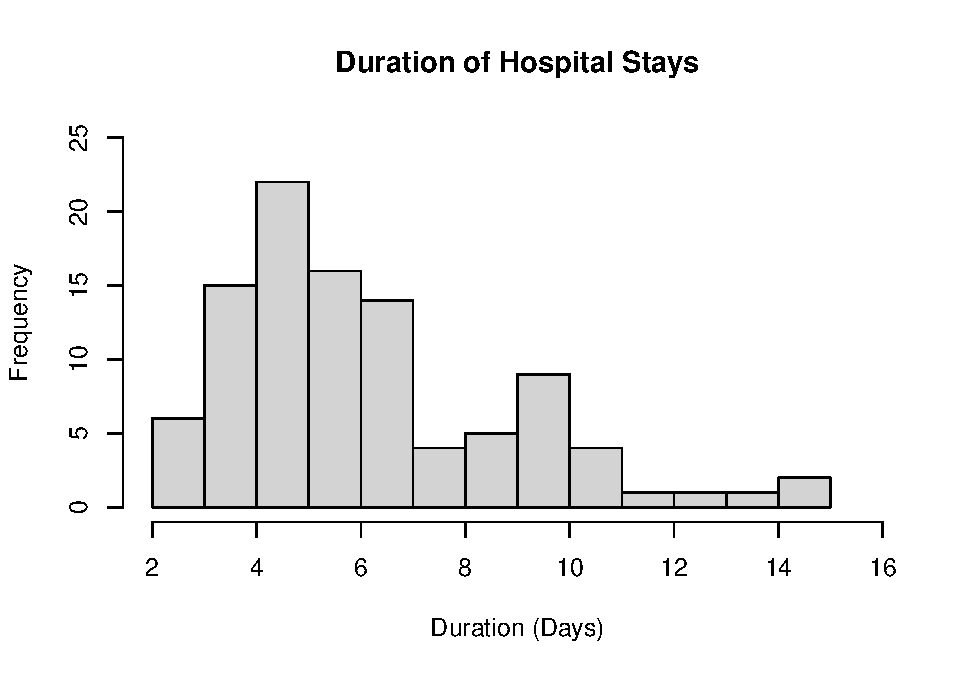
\includegraphics{Jiankun_Dong_HW1_files/figure-latex/unnamed-chunk-1-1.pdf}

Shape: ~ The data is right skewed.\\
Center: ~ The center of the data is 5 days.\\
Spread: ~ The first qualtile of the data is 4 days, and the third
quantile is 7 days. With a standard diviation of 2.74379.\\
Outliers:\\
Because the iqr of the data is 3 day, we get the lower bound -0.5 and
upper bound 11.5\\
The outliers are: 14, 13, 15, 12\\

3)\\

\begin{Shaded}
\begin{Highlighting}[]
\NormalTok{daysFrame }\OtherTok{\textless{}{-}} \FunctionTok{data.frame}\NormalTok{(}
  \AttributeTok{Mean =}\NormalTok{ daysMean,}
  \AttributeTok{Median =}\NormalTok{ daysMedian,}
  \AttributeTok{SD =}\NormalTok{ daysSD,}
  \AttributeTok{First\_Quantile =} \FunctionTok{quantile}\NormalTok{(DaysRAW}\SpecialCharTok{$}\NormalTok{Days,.}\DecValTok{25}\NormalTok{)[[}\DecValTok{1}\NormalTok{]],}
  \AttributeTok{Third\_Quantile =} \FunctionTok{quantile}\NormalTok{(DaysRAW}\SpecialCharTok{$}\NormalTok{Days,.}\DecValTok{75}\NormalTok{)[[}\DecValTok{1}\NormalTok{]],}
  \AttributeTok{Min =}\NormalTok{ daysMin,}
  \AttributeTok{Max =}\NormalTok{ daysMax}
\NormalTok{)}
\NormalTok{daysTable }\OtherTok{\textless{}{-}} \FunctionTok{kable}\NormalTok{(daysFrame,}\StringTok{"simple"}\NormalTok{)}
\end{Highlighting}
\end{Shaded}

\begin{longtable}[]{@{}rrrrrrr@{}}
\toprule\noalign{}
Mean & Median & SD & First\_Quantile & Third\_Quantile & Min & Max \\
\midrule\noalign{}
\endhead
\bottomrule\noalign{}
\endlastfoot
5.63 & 5 & 2.74379 & 4 & 7 & 2 & 15 \\
\end{longtable}

Because the outliers are all beyond the third quantile, and the
histogram is right skewed, the best value to summarize the center of
this distribution is the median 5 days.\\

The best number to describe the spread of the data is the standard
deviation 2.74379.

Problem 2:\\
4)\\
part a:\\

\begin{Shaded}
\begin{Highlighting}[]
\CommentTok{\# Question 2 {-}{-}{-}{-}{-}{-}{-}{-}{-}{-}{-}{-}{-}{-}{-}{-}{-}{-}{-}{-}{-}{-}{-}{-}{-}{-}{-}{-}{-}{-}{-}{-}{-}{-}{-}{-}{-}{-}{-}{-}{-}{-}{-}{-}{-}{-}{-}{-}{-}{-}{-}{-}{-}{-}{-}{-}{-}{-}{-}{-}{-}{-}}
\NormalTok{LessThanTen }\OtherTok{\textless{}{-}}\NormalTok{ (}\FunctionTok{pnorm}\NormalTok{(}\DecValTok{10}\NormalTok{,}\DecValTok{5}\NormalTok{,}\DecValTok{3}\NormalTok{) }\SpecialCharTok{{-}} \FunctionTok{pnorm}\NormalTok{(}\DecValTok{0}\NormalTok{,}\DecValTok{5}\NormalTok{,}\DecValTok{3}\NormalTok{))}\SpecialCharTok{/}\FunctionTok{pnorm}\NormalTok{(}\DecValTok{0}\NormalTok{,}\DecValTok{5}\NormalTok{,}\DecValTok{3}\NormalTok{,}\AttributeTok{lower.tail =} \ConstantTok{FALSE}\NormalTok{)}
\end{Highlighting}
\end{Shaded}

The percentage of the patients in hospital for less than 10 days is
94.9811103\%.\\

part b:\\

\begin{Shaded}
\begin{Highlighting}[]
\NormalTok{n }\OtherTok{\textless{}{-}} \DecValTok{35}
\NormalTok{SE }\OtherTok{\textless{}{-}} \DecValTok{3}\SpecialCharTok{/}\FunctionTok{sqrt}\NormalTok{(n)}
\NormalTok{MoreThanSix }\OtherTok{\textless{}{-}} \FunctionTok{pnorm}\NormalTok{(}\DecValTok{6}\NormalTok{,}\DecValTok{5}\NormalTok{,SE,}\AttributeTok{lower.tail =} \ConstantTok{FALSE}\NormalTok{)}\SpecialCharTok{/}\NormalTok{(}\DecValTok{1}\SpecialCharTok{{-}}\FunctionTok{pnorm}\NormalTok{(}\DecValTok{0}\NormalTok{,}\DecValTok{5}\NormalTok{,SE))}
\end{Highlighting}
\end{Shaded}

Because the sample size 35 is larger than 30, we can use the CLT. The
probability of the average of the data set being more than 6 days is
0.0243033.

\end{document}
